\documentclass[nooutcomes]{ximera}
%\documentclass[space,handout,nooutcomes]{ximera}

% For preamble materials

\usepackage{pgf,tikz}
\usepackage{mathrsfs}
\usetikzlibrary{arrows}
\usepackage{framed}
\usepackage{amsmath}
\pgfplotsset{compat=1.17}

\def\fixnote#1{\begin{framed}{\textcolor{red}{Fix note: #1}}\end{framed}}  % Allows insertion of red notes about needed edits
%\def\fixnote#1{}

\def\detail#1{{\textcolor{blue}{Detail: #1}}}   

\pdfOnly{\renewenvironment{image}[1][]{\begin{center}}{\end{center}}}

\graphicspath{
  {./}
  {chapter1/}
  {chapter2/}
  {chapter4/}
  {proofs/}
  {graphics/}
  {../graphics/}
}

\newenvironment{sectionOutcomes}{}{}


%%% This set of code is all of our user defined commands
\newcommand{\bysame}{\mbox{\rule{3em}{.4pt}}\,}
\newcommand{\N}{\mathbb N}
\newcommand{\C}{\mathbb C}
\newcommand{\W}{\mathbb W}
\newcommand{\Z}{\mathbb Z}
\newcommand{\Q}{\mathbb Q}
\newcommand{\R}{\mathbb R}
\newcommand{\A}{\mathbb A}
\newcommand{\D}{\mathcal D}
\newcommand{\F}{\mathcal F}
\newcommand{\ph}{\varphi}
\newcommand{\ep}{\varepsilon}
\newcommand{\aph}{\alpha}
\newcommand{\QM}{\begin{center}{\huge\textbf{?}}\end{center}}

\renewcommand{\le}{\leqslant}
\renewcommand{\ge}{\geqslant}
\renewcommand{\a}{\wedge}
\renewcommand{\v}{\vee}
\renewcommand{\l}{\ell}
\newcommand{\mat}{\mathsf}
\renewcommand{\vec}{\mathbf}
\renewcommand{\subset}{\subseteq}
\renewcommand{\supset}{\supseteq}
%\renewcommand{\emptyset}{\varnothing}
%\newcommand{\xto}{\xrightarrow}
%\renewcommand{\qedsymbol}{$\blacksquare$}
%\newcommand{\bibname}{References and Further Reading}
%\renewcommand{\bar}{\protect\overline}
%\renewcommand{\hat}{\protect\widehat}
%\renewcommand{\tilde}{\widetilde}
%\newcommand{\tri}{\triangle}
%\newcommand{\minipad}{\vspace{1ex}}
%\newcommand{\leftexp}[2]{{\vphantom{#2}}^{#1}{#2}}

%% More user defined commands
\renewcommand{\epsilon}{\varepsilon}
\renewcommand{\theta}{\vartheta} %% only for kmath
\renewcommand{\l}{\ell}
\renewcommand{\d}{\, d}
\newcommand{\ddx}{\frac{d}{dx}}
\newcommand{\dydx}{\frac{dy}{dx}}


\usepackage{bigstrut}


%\usepackage{tikz}


\title{Measurement}
\author{Brad Findell}
\begin{document}
\begin{abstract}
Short-answer problems about measurement. 
\end{abstract}
\maketitle




\section{Numbers, Units, and Quantities}
In this section, we develop and explain the algebra of measurement calculations and unit conversions. 

\begin{question}
Brad measured his driveway to be 21 feet long.  How long is it in yards?  
$\answer{7}$ yards.  
\end{question}

We all know that 3 feet and 1 yard express the same length.  Let's write an equation to express this equality of lengths: 
\[
3\;\textrm{ft} = 1\;\textrm{yd}
\]

Here is a picture illustrating this idea:  

\begin{image}
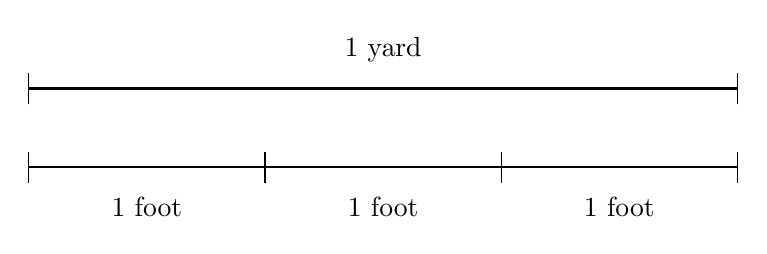
\begin{tikzpicture}[xscale=1]
\draw [thick] (0,1) -- (9,1);
\draw (0,1-.2) -- (0, 1+.2);
\draw (9,1-.2) -- (9,1+ .2);
\draw [thick] (0,0) -- (9,0);
\draw (0,-.2) -- (0, .2);
\draw (3,-.2) -- (3, .2);
\draw (6,-.2) -- (6, .2);
\draw (9,-.2) -- (9, .2);
\node[align=center] at (4.5,1.5)%
{1 yard};
\node[align=center] at (1.5,-.5)%
{1 foot};
\node[align=center] at (4.5,-.5)%
{1 foot};
\node[align=center] at (7.5,-.5)%
{1 foot};
\end{tikzpicture}
\end{image}

\begin{question}
The equation $3\;\textrm{ft} = 1\;\textrm{yd}$ seems to suggest that you \wordChoice{\choice[correct]{multiply}\choice{divide}} feet by 3 to get yards.  But when converting feet to yards in the question above you \wordChoice{\choice{multiplied}\choice[correct]{divided}} the number of feet by 3.  

Why do these answers appear to be opposites of each other?  
\end{question}

The resolution of this conundrum requires that we distinguish numbers (e.g., 21) from units (e.g., feet).  Quantities measuring, say, length, weight, or speed involve both numbers and units, but the numbers behave differently from the units, as we see in the example above.  

With a little algebraic manipulation, the equation $3\;\textrm{ft} = 1\;\textrm{yd}$ is equivalent to the following equations:  
\[
\frac{3\;\textrm{feet}}{1\;\textrm{yard}} = 1\qquad \textrm{and}\qquad \frac{1\;\textrm{yard}}{3\;\textrm{feet}} = 1.
\]
In both equations, the 1 on the right is ``dimensionless'' in the sense that it is without units.  Think of it as a scale factor of 1, which leaves lengths unchanged.  These equations are useful for demonstrating the conversion from feet to yards and vice versa:  

%\begin{align*}
%21\textrm{ feet} &= 21\; \textrm{feet} \\
%21\textrm{ feet} &= 21\textrm{ feet} \\
%21\textrm{ feet} &= 21\ \textrm{feet} \\
%21\textrm{ feet} &= 21\, \textrm{feet} \\
%21\textrm{ feet} &= 21\: \textrm{feet} 
%\end{align*}

\[
21\;\textrm{feet} = 21\;\cancel{\textrm{feet}} \cdot \frac{{1\;\textrm{yard}}}{3\;\cancel{\textrm{feet}}} = 7\;\textrm{yards}
\]

\[
7\;\textrm{yards} = 7\;\cancel{\textrm{yards}} \cdot \frac{{3\;\textrm{feet}}}{1\;\cancel{\textrm{yard}}} = 
21\;\textrm{feet}
\]

These examples illustrate an \emph{algebra of units}, in which units behave much like algebraic variables.  In both conversions, we multiply a quantity by a dimensionless 1, so that the calculation doesn't change the amount that the quantity represents.  The cancellation of units helps to confirm that we are doing the calculation correctly.  

At a conceptual level, this algebra of units helps illuminate how the numbers and units behave in apparently opposite ways:  

\begin{itemize}
\item Yards are three times as big as feet, so there are one-third as many in a given length.  
\item Feet are one-third the size of yards, so there are three times as many in a given length.  
\end{itemize}

Thus, we must be careful to consider whether the letters represent numbers or units.  


\section{Square Units and Cubic Units}
Because $3\;\textrm{ft} = 1 \;\textrm{yd}$, it is tempting to conclude that $3\;\textrm{square feet} = 1 \;\textrm{square yards}$.  But \dots

\begin{question}
What is a square foot?  What is a square yard? 
\begin{freeResponse}
\begin{hint}
A square foot is the area of a square that measures 1 foot by 1 foot.  A square yard is the area of a yard that measures 1 yard by 1 yard. 
\end{hint}
\end{freeResponse}
\end{question}

\begin{question}
How many square feet are in a square yard?  $\answer{9}$.  

Provide a geometric explanation. Provide an explanation based on the algebra of units. 
\begin{freeResponse}
\begin{hint}
From pictures of a square yard and a square foot, it is not hard to see that it takes 9 square feet to cover 1 square yard.  (Draw pictures.)
\end{hint}
\begin{hint}
\[
1\;\textrm{square yard} = 1\;\textrm{yard}^2 = 1\cdot(3\;\textrm{feet})^2 = 9\;\textrm{feet}^2 = 9\;\textrm{square feet}
\]
\end{hint}
\end{freeResponse}
\end{question}


\end{document}
